\subsubsection{Selenium}
Selenium ist ein OpenSource-Framework für Abnahme-, System und
Funktionstests von Web-Applikationen. Selenium kann auf
unterschiedliche Weise eingesetzt werden:
\begin{itemize}
\item in einem Browser: Selenium Core (unterschiedliche Browser)
  eventuell in Ergänzung mit Selenium IDE (Firefox)
\item als Proxy-Server: Selenium Remote Control (RC) für die Durchführung
  automatisierter Web-Tests in unterschiedlichen Programmiersprachen
  (Java, C\#, Perl, Python, Ruby)
\end{itemize}
\newslide
Beispielsweise in Kombination mit JUnit:
\begin{lstlisting}[language=java]
public class SeleniumWebTest extends TestCase {
  private DefaultSelenium selenium;

  public void setUp() throws Exception {
    super.setUp();
    selenium = new DefaultSelenium("localhost", 4444,
                                   "*firefox",
                                   "http://localhost:8080/");
    selenium.start();
  }

  public void tearDown() throws Exception {
    selenium.stop();
    super.tearDown();
  }

  public void testHelloWorld() throws Exception {
    try {
      selenium.open("http://localhost:8080/hitchhikers-guide");
      assertEquals("Hello World", selenium.getText("//h2"));
    } catch (SeleniumException ex) {
      fail(ex.getMessage());
      throw ex;
    }
  }
}
\end{lstlisting}
\newslide
In einem Maven-Projekt (genauer in einem von Maven verwalteten Projekt)
ergänzt man das POM-File mit dem folgenden Dependency-Element
\begin{lstlisting}[language=xml,
  morekeywords={dependency,groupId,artifactId,version,scope,enabled}]
<dependency>
   <groupId>
      org.openqa.selenium.client-drivers
   </groupId>
   <artifactId>selenium-java-client-driver</artifactId>
   <version>0.9.2</version>
   <scope>test</scope>
</dependency>
\end{lstlisting}
\newslide
Dazu wird ein spezielles Maven-Repository benötigt:
\begin{lstlisting}[language=xml,
  morekeywords={repositories,repository,id,name,url,layout,snapshots,releases}]
 <repositories>
        <repository>
            <id>openqa</id>
            <name>OpenQA Repository</name>
            <url>http://maven.openqa.org</url>
            <layout>default</layout>
            <snapshots>
                <enabled>false</enabled>
            </snapshots>
            <releases>
                <enabled>true</enabled>
            </releases>
        </repository>
  </repositories>
\end{lstlisting}
\newslide
sowie die beiden folgenden Plugins:
\begin{lstlisting}[language=xml,
  morekeywords={plugin,groupId,artifactId}]
<plugin>
 <groupId>org.codehaus.mojo</groupId>
 <artifactId>selenium-maven-plugin</artifactId>
</plugin>
<plugin>
  <groupId>org.mortbay.jetty</groupId>
  <artifactId>maven-jetty-plugin</artifactId>
</plugin>
\end{lstlisting}
\newslide
Nun kann in einem Terminal die Web-Applikation gestartet werden:
\begin{lstlisting}
  % mvn jetty:run
\end{lstlisting}
in einem zweiten Terminal der Selenium-Server:
\begin{lstlisting}
  % mvn selenium:start-server
\end{lstlisting}
und schliesslich in einem dritten Terminal der Test:
\begin{lstlisting}
  mvn test
\end{lstlisting}
Für weitere Vereinfachung siehe

\href{http://wiki.foochal.org/index.php/Maven_Selenium#Simple_selenium_java_unit_test}
{wiki.foochal.org/index.php/Maven\_Selenium\#Simple\_selenium\_java\_unit\_test}

und

\href{http://binil.wordpress.com/2006/12/08/automated-smoke-tests-with-selenium-cargo-testng-and-maven/}
{binil.wordpress.com/2006/12/08/automated-smoke-tests-with-selenium-cargo-testng-and-maven/}
%
\begin{figure}[H]
\begin{center}
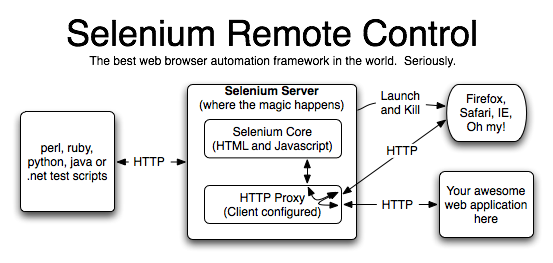
\includegraphics[width=\linewidth]{qm/selenium-rc}
\end{center}
\caption{Selenium Remote Control
  (Quelle \href{http://www.openqa.org/selenium-rc/tutorial.html}
   {www.openqa.org/selenium-rc/tutorial.html})}
\end{figure}
\begin{figure}[H]
\begin{center}
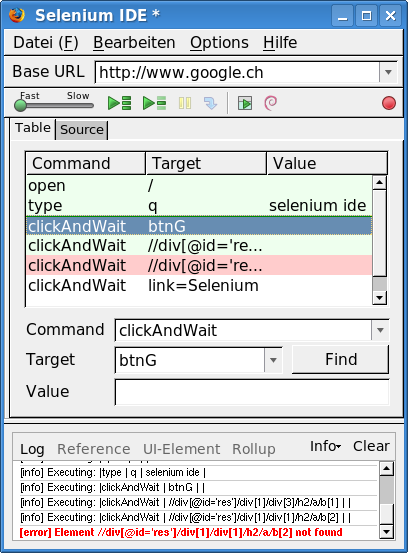
\includegraphics[width=0.5\linewidth]{qm/selenium-ide}
\end{center}
\caption{Selenium IDE als Firefox Plugin}
\end{figure}
%
